\section{Rivelatore di fronti d'onda}
\begin{wrapfigure}[14]{r}[0pt]{54mm}
	\caption{Schema del circuito rilevatore di fronti di salita/discesa}
	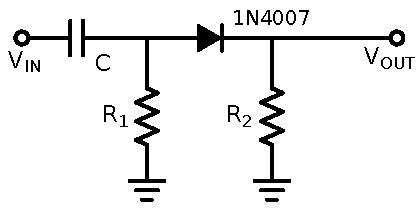
\includegraphics[width=54mm]{schema_peak_detector.pdf}
	\label{fig:schema_peak_detector}
\end{wrapfigure}

Il circuito riportato in Fig. \ref{fig:schema_peak_detector} rappresenta lo schema del rivelatore di fronti d'onda utilizzato il laboratorio. Come vediamo, se si considera solo la parte a monte del diodo, esso risulta un semplice filtro passa alto. Particolarità di tale filtro è il suo utilizzo come derivatore. Infatti, se la capacità C e la resistenza R sono piccole:


$$ I=\frac{V_{out}'(t)}{R_1}=C\frac{d}{dt}(V_{in}(t)-V_{out}'(t)) \approx C \frac{dV_{in}(t)}{dt} $$

\begin{equation} 
\Rightarrow V_{out}(t) \approx R_1C \frac{dV_{in}(t)}{dt} 
\label{derivatore}
\end{equation}

L'inserimento del diodo a valle di tale derivatore permette il passaggio dei soli segnali positivi/negativi (in base al verso del diodo stesso). Per osservare il funzionamento come rivelatore di fronti d'onda abbiamo alimentato il circuito con una forma d'onda quadra alla frequenza di $100 \si{\hertz}$ e tensione $V_{PP}=10 \si{\volt}$. L'onda quadra ha la particolarità di essere una funzione a tratti. Utilizzando capacità e resistenze molto piccole, il circuito rileverà i punti in cui la derivata tende ad infinito mentre nei tratti in cui la derivata è uguale a zero non lascerà passare nessun segnale (vedi Eq. \ref{derivatore}).

E' stata fissata una resistenza $R_2=(1000.4 \pm 0.2) \si{\ohm}$. 

Poichè a parità di segnale in ingresso $V_{in}$ il segnale in uscita dipende sia da $R_1$ che da $C$, abbiamo deciso di effettuare due campionamenti, bloccando una delle due variabili e facendo variare l'altra. Riportiamo nei due seguenti grafici i dati sperimentali da noi ottenuti.


$$*grafici*$$


Come vediamo, i valori di tensione $V_{out}^{MAX}$ in entrambi i grafici tendono a valori bassi sia quando valori di resistenza e capacità sono piccoli sia quando sono grandi. Da Eq. (\ref{derivatore}) ci si aspetterebbe che all'aumentare di $R_1$ e $C$ aumenti anche $V_{out}$. Dobbiamo tuttavia ricordare l'approssimazione fatta per ricavare Eq. (\ref{derivatore}). Infatti avevamo assunto che sia capacità che resistenza fossero molto piccole. Evidentemente essa non è più valida per valori troppo grandi di queste due variabili. Ricordiamo anche che sebbene teoricamente l'onda quadra abbia derivata infinita nei punti di discontinuità, non è possibile in laboratorio generare un segnale discontinuo con questa caratteristica. Il valore $\frac{dV_{in}(t)}{dt}=\gamma$  sarà dunque ben definito e potrà essere assunto in prima approssimazione mediamente costante. Per valori piccoli di $C$ ed $R_1$ avremo dunque una legge del tipo $V_{out}^{MAX}= RC \gamma$. \`E dunque evidente che per valori di $R_1\rightarrow 0$ o $C\rightarrow 0$ il valore di tensione in uscita tenderà a zero.

Per valori di resistenza e capacità grandi non possiamo fare l'approssimazione di derivatore e dunque non possiamo più ricondurci all'equazione sopra calcolata. Per valori di capacità molto grandi osserveremo una tensione in uscita $V_{out}(t)=I(t) R_1$. Ma $I(t)$ sarà uguale alla corrente di che scorre in un circuito RC. Quando C diventa grande, il condensatore non riuscirà nemmeno a caricarsi completamente e dunque avremo un valore di tensione $V_{out}$ che decresce aumentando C. Analogamente, quando R diventa molto grande, la corrente che può scorrere nel circuito diventa piccola e dunque il condensatore non riuscirà a caricarsi completamente. Avremo anche in questo caso che la tensione $V_{out}$ decresce aumentando R. Riportiamo per completezza due grafici dei dati visualizzati sull'oscilloscopio. Il primo con $C$ ed $R_1$ piccoli mentre il secondo con $C$ ed $R_1$ abbastanza grandi per apprezzare l'andamento della tensione indotto dalla presenza del condensatore. 


\begin{figure}[h]
\center
	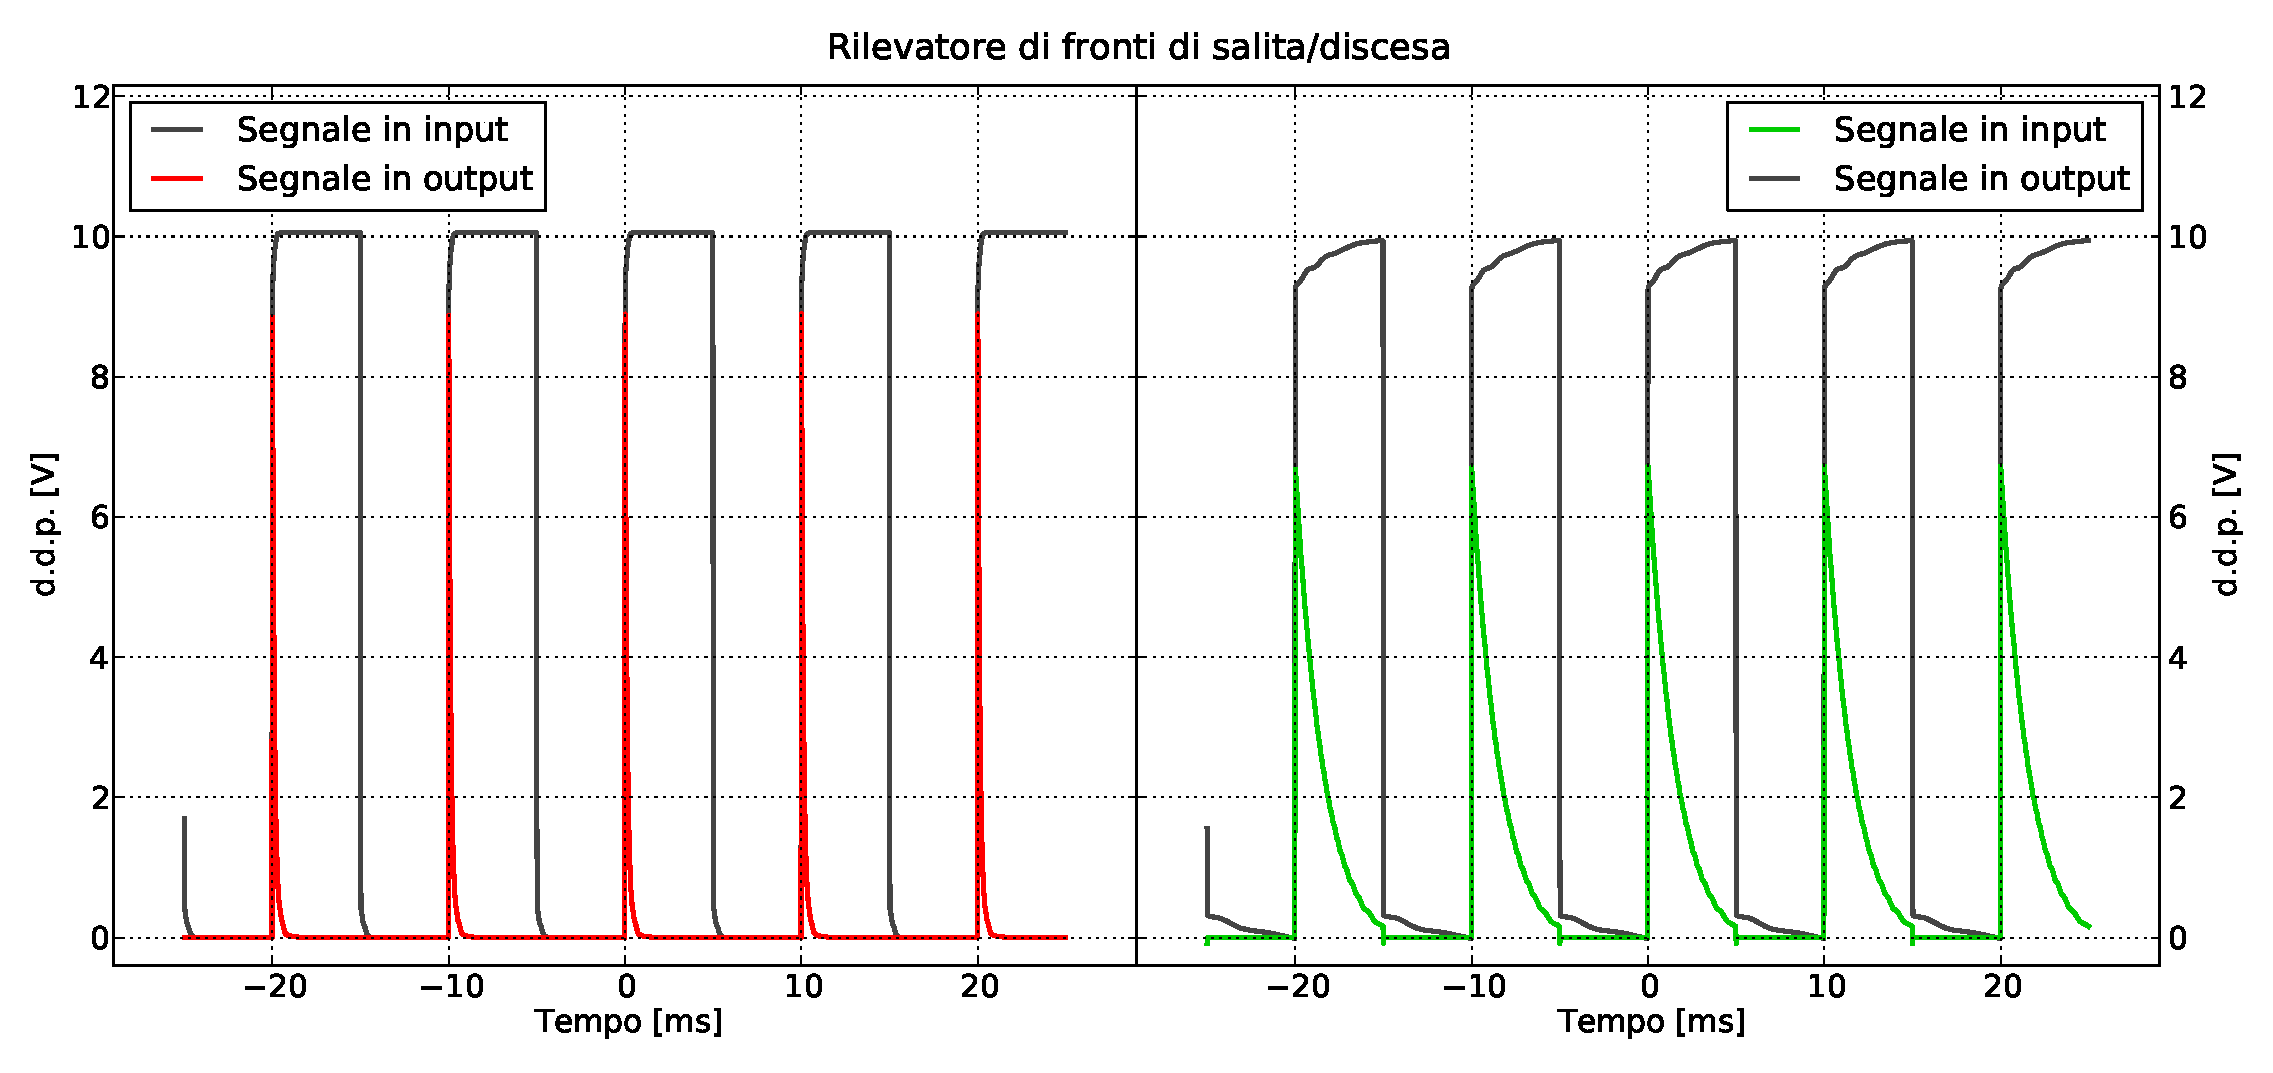
\includegraphics[width=\textwidth]{peaks(2).pdf}
	\caption{.}
	\label{fig:peaks}
\end{figure}

\section{Diodo Zener}
Poichè il funzionamento del diodo zener è in inversa, abbiamo campionato solo la caratteristica V-I in inversa. Ricordiamo che a differenza di un diodo come quello utilizzato nell'esperienza precedente, il valore di corrente in funzione della tensione in un diodo zener, una volta raggiunto il range operativo, è lineare. Ovvero esiste una ``resistenza'' \footnote{Non è possibile definirla resistenza in quanto essa è ben definita solo per un insieme ristretto di valori di tensione diverso da tutta l'asse reale}, $R_d$, t.c. $V=R_d I$.

Utilizzando la breadboard come supporto, abbiamo creato un circuito composto dal generatore di tensione continua (DC $\pm \SI{25}{\volt}$), il diodo zener e il multimetro digitale in modalità amperometro. Aumentando progressivamente la tensione, abbiamo letto sull'amperometro i valori della corrente che attraversava il circuito.
Facendo attenzione che la corrente non superasse il valore di \SI{70000}{\milli\ampere} abbiamo campionato l'asse negativo del grafico. Il risultato è esposto in Fig. \ref{fig:VI_zener}.

\begin{figure}[h]
\center
	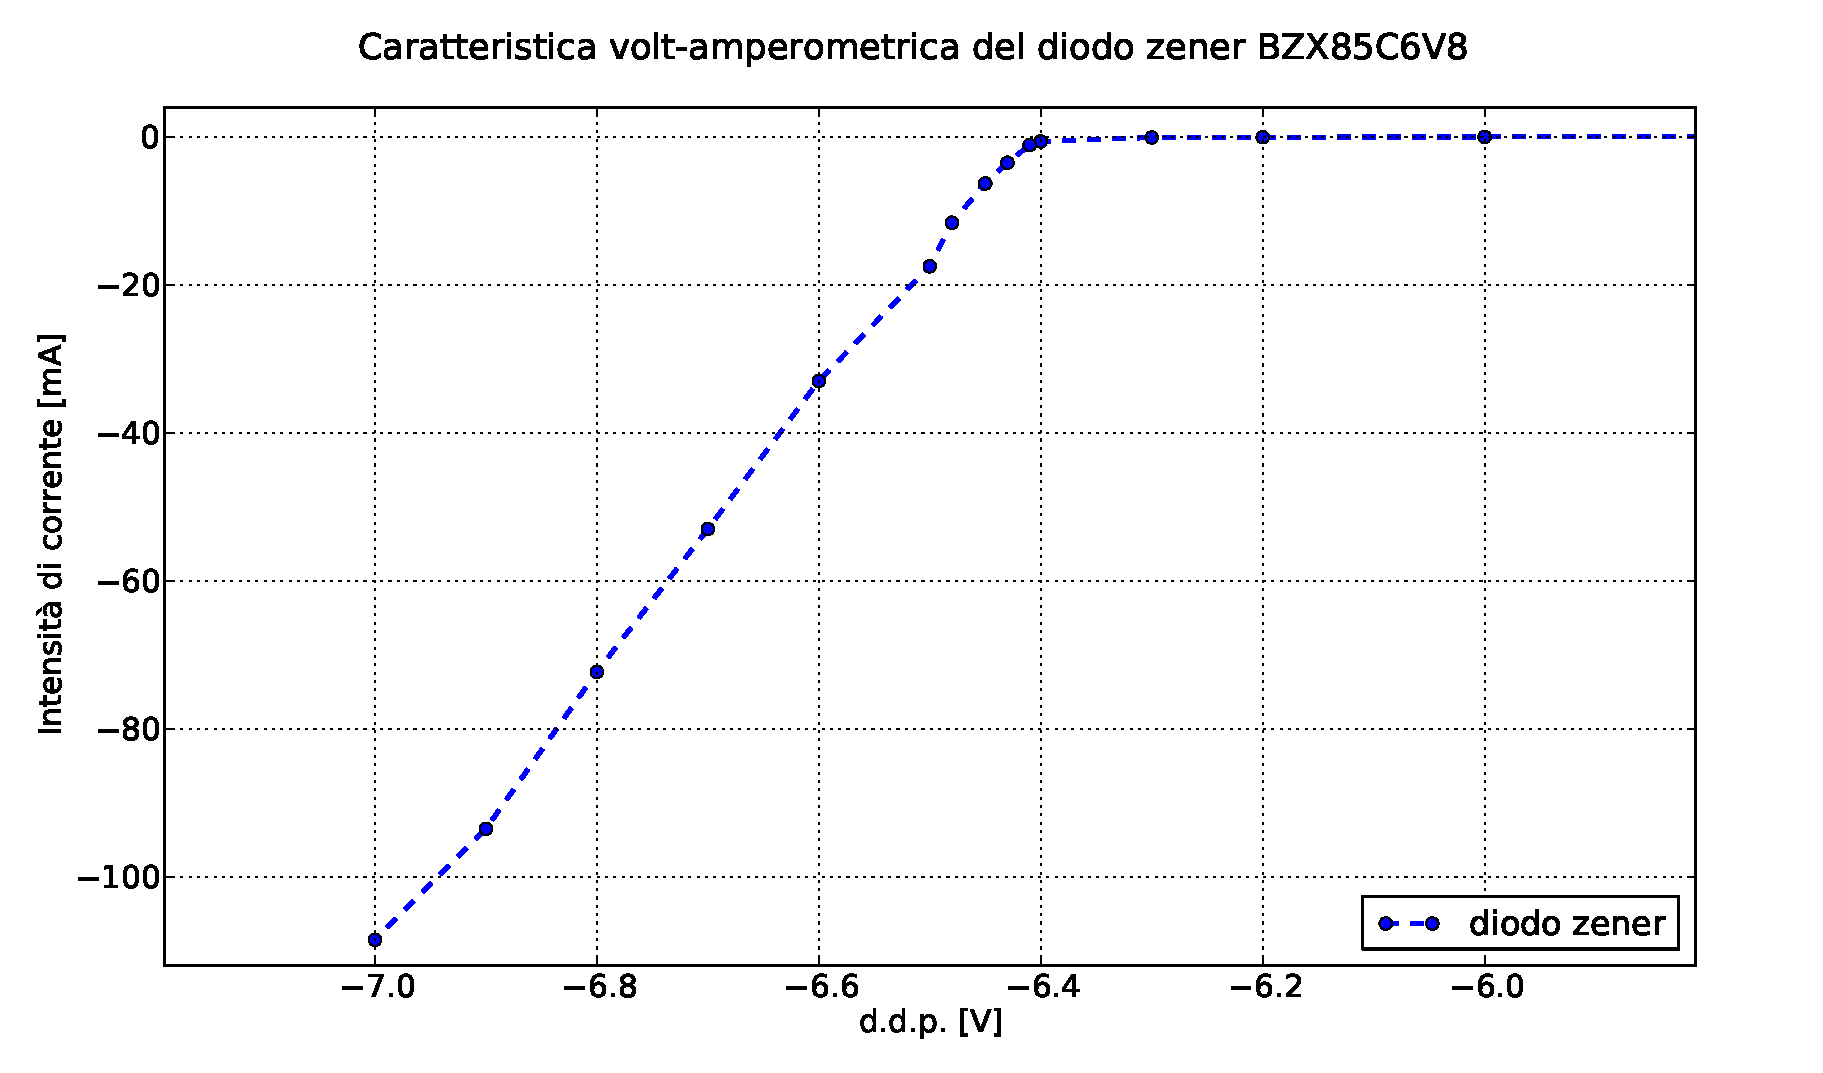
\includegraphics[width=0.66\textwidth]{VI_zener.pdf}
	\caption{Caratteristica volt-amperometrica del diodo zener BZX85C6V8. I valori di corrente relativi a tensioni comprese tra quelle graficate e l'origine degli assi sono stati esclusi perché poco importanti.}
	\label{fig:VI_zener}
\end{figure}
\newpage
%\begin{minipage}[t]{width=1\textwidth}
Dai dati ottenuti è stato possibile calcolare la resistenza dinamica del diodo, ovvero:

\begin{wrapfigure}[14]{r}[0pt]{50mm}
	\caption{Schema del circuito in cui il diodo Zener BZX85C6V8 è usato come stabilizzatore di tensione.}
	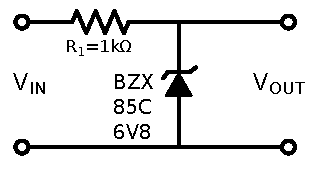
\includegraphics[width=50mm]{schema_zener.pdf}
	\label{fig:schema_zener}
\end{wrapfigure}

\begin{equation}
R_d=\frac{\Delta V}{\Delta I}
\label{scemopagliaccio}
\end{equation}

Eseguita la media pesata dei vari $R_d$, otteniamo come risultato
$$R_d= * \pm *$$

Nella seconda parte dello studio del diodo zener, abbiamo analizzato il suo funzionamento come stabilizzatore di tensione. Anzitutto è stato montato il circuito riportato in Fig. \ref{fig:schema_zener} con $R= \pm $.  Dallo studio della caratteristica V-I del diodo abbiamo stimato che esso può essere utilizzato come stabilizzatore di tensione da $7000 V$ fino a quando la potenza massima dissipata lo permette. 

Riportiamo in Fig. \ref{fig:stabilizer} i dati da noi ottenuti.
%\end{minipage}

\begin{figure}[h]
\center
	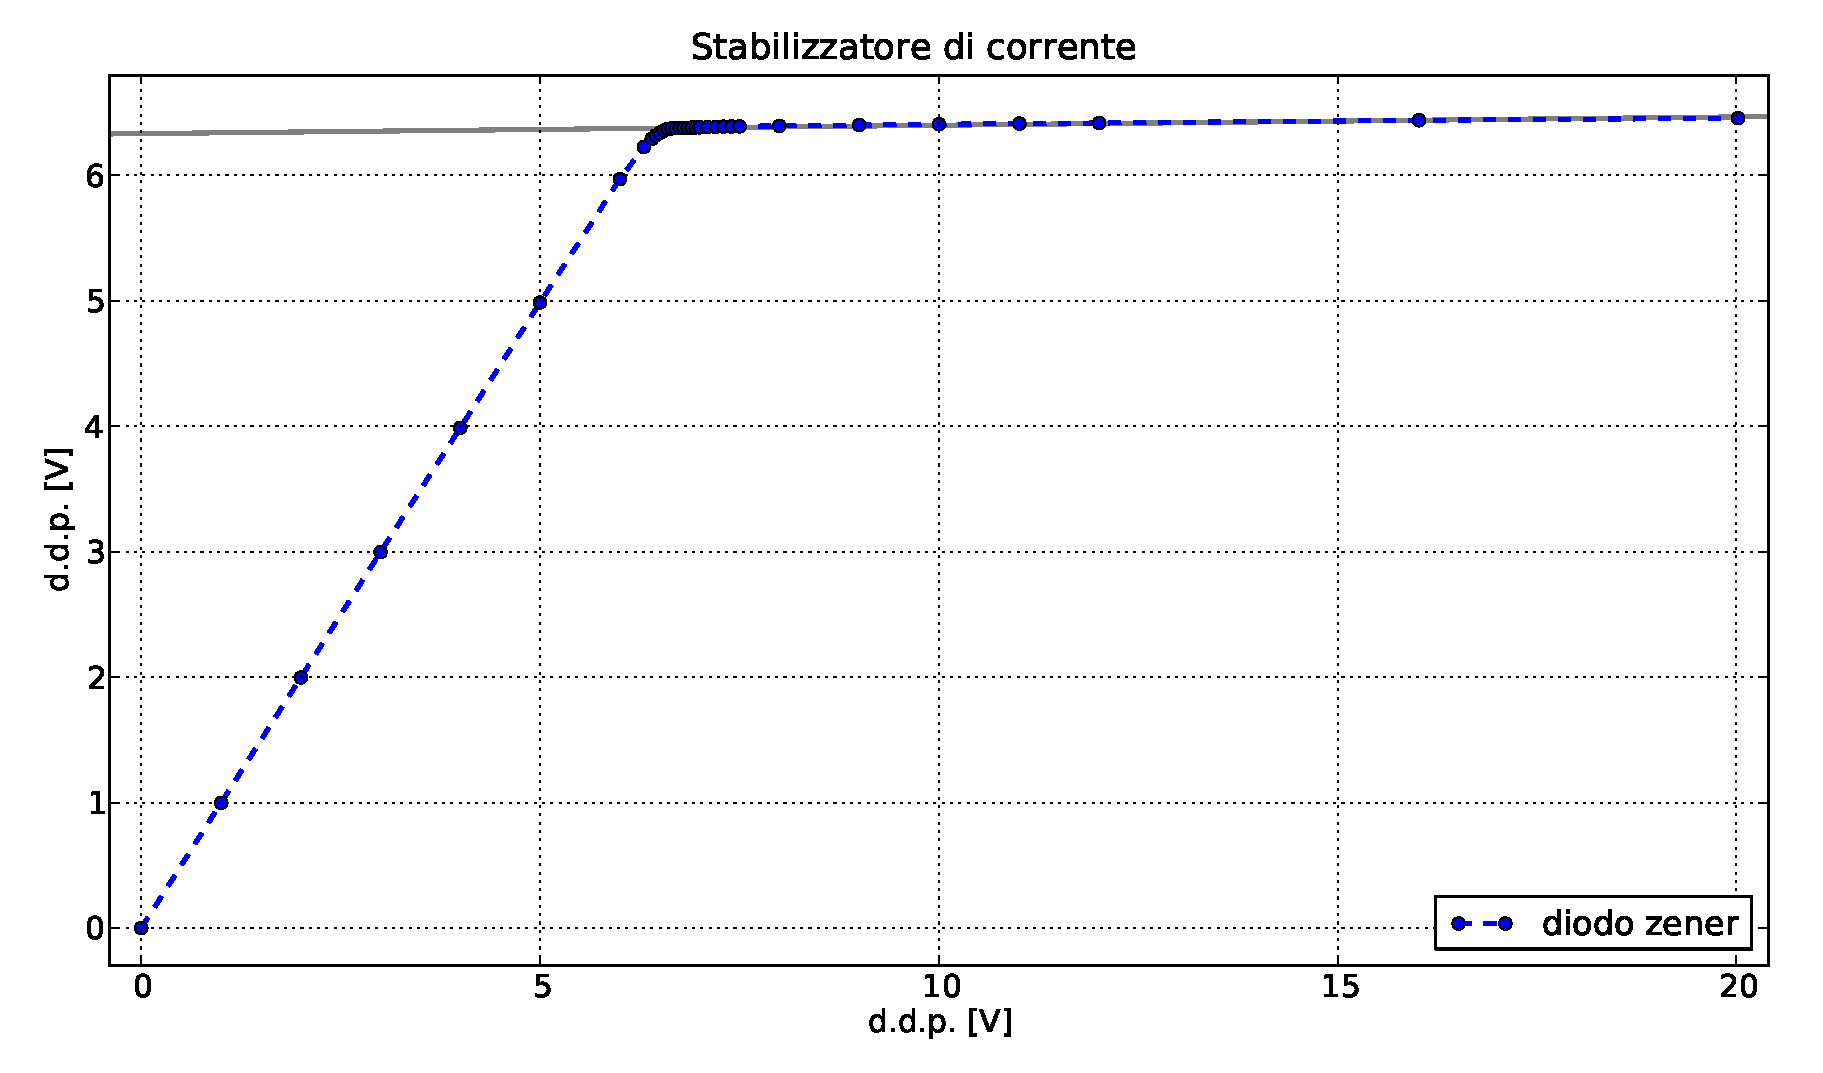
\includegraphics[width=0.66\textwidth]{stabilizer.pdf}
	\caption{.}
	\label{fig:stabilizer}
\end{figure}

\`E stato dunque calcolato il rapporto di stabilizzazione teorico dalla formula: 

\begin{equation}
{R_S}_{teo}=\frac{R_d}{R+R_d}
\label{RS_teo}
\end{equation}

$${R_S}_{teo}= * \pm *$$

e confrontato con la media pesata di quelli sperimentali $\frac{\Delta V_{out}}{\Delta V_{in}}$.

$${R_S}_{exp}= * \pm *$$
 